\documentclass[a4paper,17pt]{extarticle}
\usepackage{tikz,mathspec,makecell,graphicx,qrcode}
\usepackage[russian]{babel}
\usepackage[top=1cm,bottom=0cm,outer=1.8cm,inner=1.8cm]{geometry}
\parindent=0.6in \parskip=2.8mm

\setmainfont[
	Path = f/,
	BoldFont=lb.ttf,
	ItalicFont=li.ttf,
	BoldItalicFont=lbi.ttf
		]{l.ttf}
\setsansfont[
	Path = f/,
	BoldFont=lb.ttf,
	ItalicFont=li.ttf,
	BoldItalicFont=lbi.ttf
		]{l.ttf}
		
\setmathfont(Digits)[Path = f/]{l.ttf}
\setmathfont(Latin)[Path = f/]{li.ttf}
\newcommand{\xx}{$\times\times$}


\begin{document} \thispagestyle{empty}

\begin{center} \begin{tabular}{ccc}
	\makecell[c]{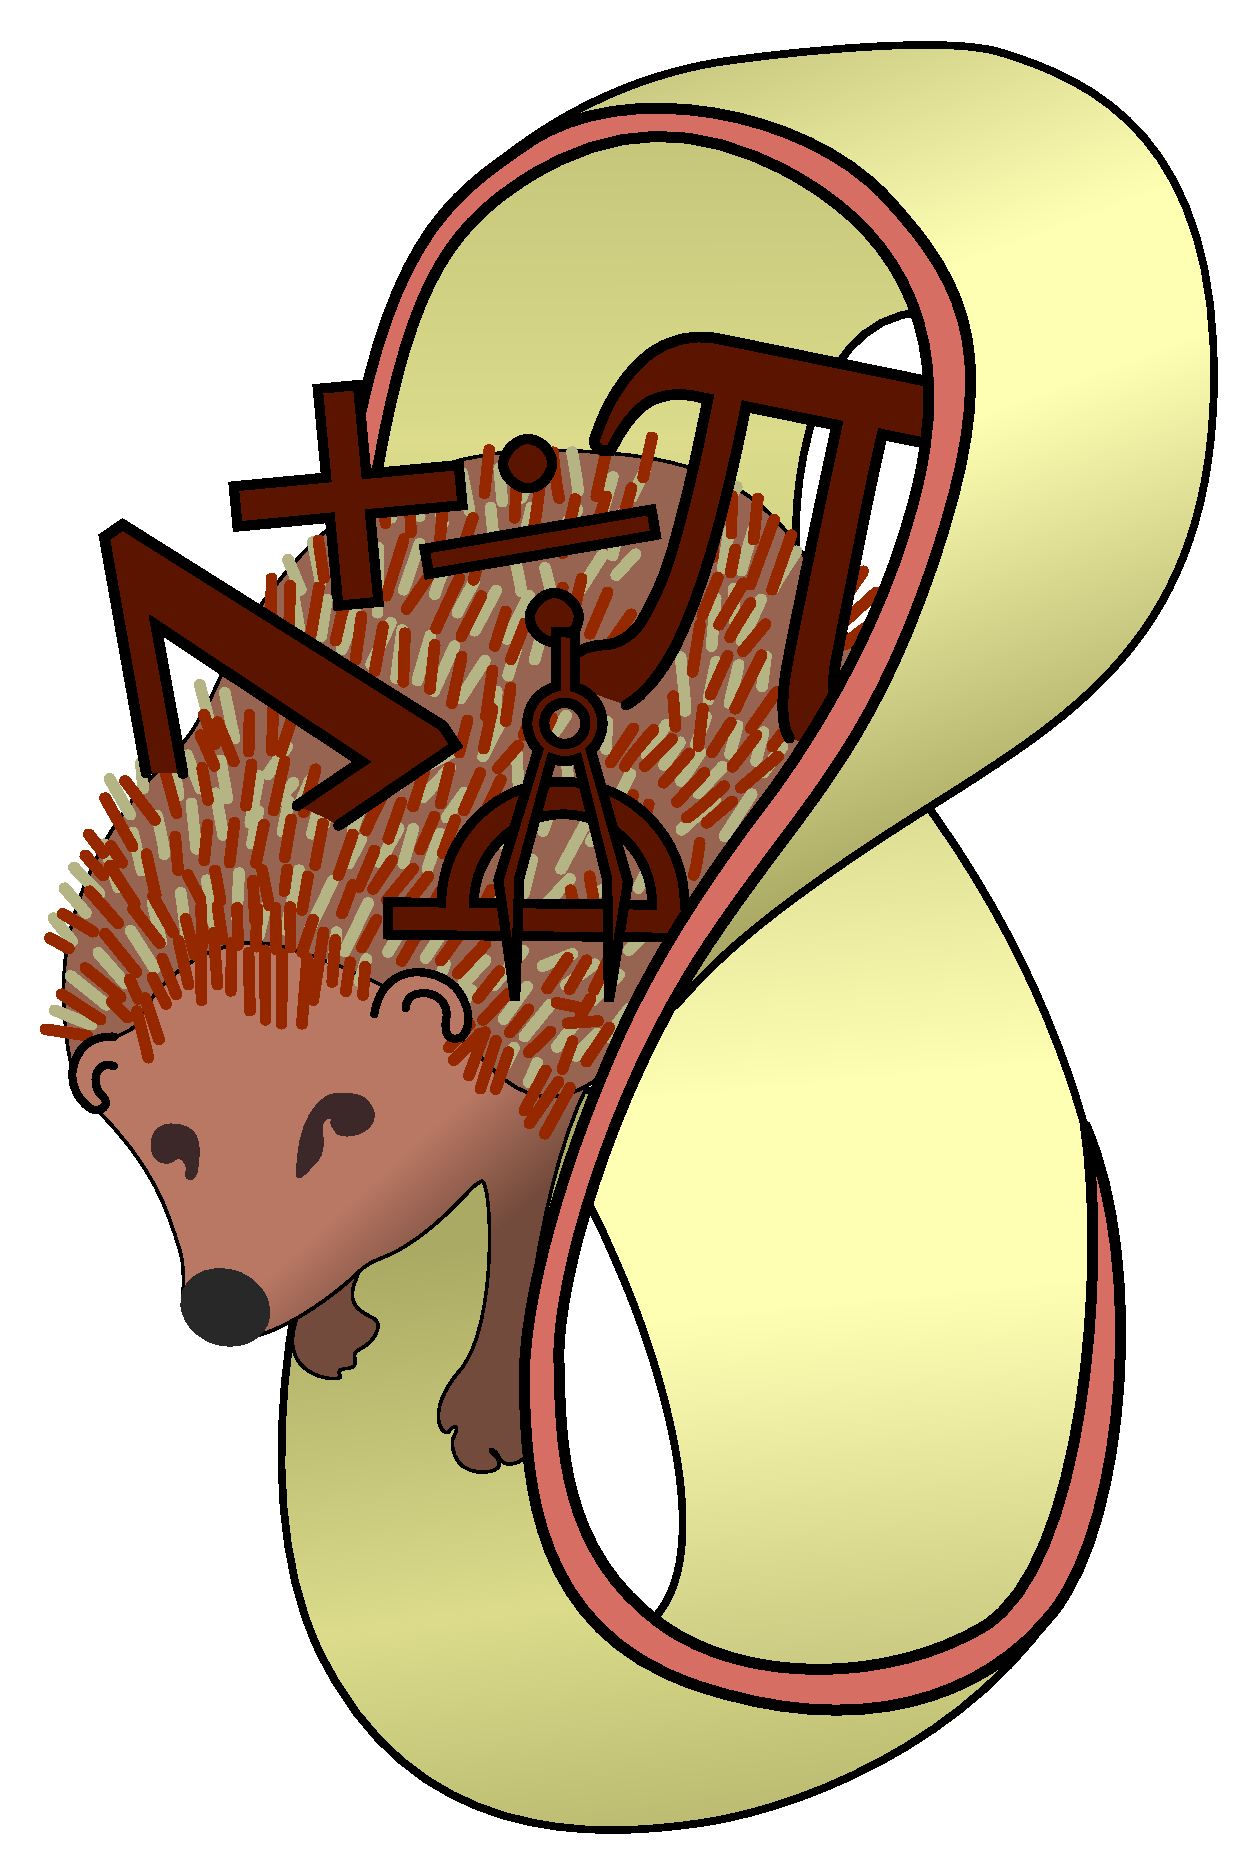
\includegraphics[height=3.7cm]{h}} &
	\hspace{0.7cm} &
	\makecell[c]{
\includegraphics[height=1.75cm]{funds}}
\end{tabular}

\begin{tabular}{l}
	\makecell[l]{{\large\bf Приглашаем на семинары,}\\
		{\large\bf посвящённые олимпиаде}\\
		{\large\bf «Математика НОН-СТОП»}}
\end{tabular}\end{center}

«Математика НОН-СТОП» — уникальная олимпиада, направленная на привлечение интереса школьников не только к олимпиадным задачам как таковым, но и к решению проблем глубокого исследовательского характера.

Организаторы олимпиады проводят серию семинаров, на которых расскажут об олимпиадах и их задачах. Мы надеемся, что семинары привлекут детей и взрослых к участию в «Математике НОН-СТОП», помогут привить детям интерес к математике и конкурсам.\vspace{-3mm}

\begin{center} \begin{tabular}{ll}
	—%17 мая, 18:00
		\phantom{проб} &
		\makecell[l]{Занимательная лекция \\ по математике} \\
	\vspace{-4mm} \\
	—%17 мая, 22:00
		\phantom{проб} &
		\makecell[l]{Решение избранных \\ задач олимпиад}
\end{tabular} \end{center}

Также будут сделаны доклады, полезные преподавателям, которые хотели бы принимать участие в проведении олимпиад или вести олимпиадную математику у своих учеников.\vspace{-3mm}

\begin{center} \begin{tabular}{ll}
	—%18 мая, 18:00
		\phantom{проб} &
		\makecell[l]{Принципы составления задач \\ олимпиад и турниров} \\
	\vspace{-4mm} \\
	—%18 мая, 22:00
		\phantom{проб} &
		\makecell[l]{Как учить олимпиадной мате- \\ матике: программа кружка}
\end{tabular} \end{center}


\begin{center}
	Ждём вас на семинарах!%\\[0.3cm]
%	{\bf\large rs.mathnonstop.ru}
\end{center}

\tikz[remember picture,overlay]{
	\node[opacity=0.28,inner sep=0pt] at (current page.center)
	{
\includegraphics[width=\paperwidth,height=\paperheight]{h-page}};
}
\clearpage

\end{document}
